\documentclass[11pt,a4paper]{article}
\usepackage[T1]{fontenc}
\usepackage[utf8]{inputenc}
\usepackage[french]{babel}
\usepackage{lmodern}
\usepackage[margin=2.2cm]{geometry}
\usepackage{amsmath,amssymb}
\usepackage{booktabs}
\usepackage{graphicx}
\usepackage{float}
\usepackage[hidelinks]{hyperref}

\setlength{\emergencystretch}{3em}
\newcommand{\code}[1]{\texttt{#1}}

\title{Moteur d'échecs matriciel sur GPU, incrément 2\\[2pt]
\large Qualité coup par coup, tri des coups, vagues adaptatives, pendule\\
\normalsize Rapport d'incrément et plan du suivant}
\author{Projet \code{chess-gpu}, branche \code{claude/zen-pasteur-vjg9yx}}
\date{24 novembre 2026}

\begin{document}
\maketitle

\begin{abstract}
L'incrément 1 avait conclu que la profondeur limite la force de notre moteur et que l'alpha-bêta
par lots gagne 2 à 3 demi-coups à temps égal. L'incrément 2 suit son plan, avec trois agents
travaillant en parallèle sur des copies isolées du dépôt.
\begin{itemize}
\item \textbf{Une analyse coup par coup par Stockfish}, à la manière de Lichess, assortie d'un
filtre de qualité déterministe à lancer avant tout match.
\item \textbf{Un tri des coups MVV/LVA et des vagues adaptatives} dans l'alpha-bêta exact.
\item \textbf{Une pendule bornée}, avec résultat partiel sûr, refus de la répétition et journal par
coup.
\end{itemize}
Sur 5\,336 coups, l'analyse montre que nos parties se perdent à la sortie de l'ouverture : le coup
décisif tombe au coup 10 en médiane. Sur une RTX PRO 6000, le filtre de qualité fait passer la
perte moyenne du coup choisi de 35{,}9 à 29{,}6~cp. Le duel de 200 parties en 10~s~+~0{,}1~s, avec
ouvertures appariées et couleurs inversées, donne au nouveau moteur \textbf{67{,}5~\% des points,
soit $+127$ Elo [$+90$ ; $+167$]} contre l'alpha-bêta de l'incrément 1.
\end{abstract}

\tableofcontents

\section{Point de départ et organisation}
L'incrément 1 (\code{docs/etudes/2026-11-24\_increment1-gpu/}) a livré la génération de coups sur
GPU, un alpha-bêta par lots exact et des matchs contre Stockfish, avec un score de 7{,}5/14 en
conditions de calibration. Son plan, partagé par les trois agents consultés, plaçait en tête un
filtre de qualité, le tri des coups, des vagues adaptatives et la gestion du temps.

Trois agents ont travaillé en parallèle, chacun dans une copie isolée du dépôt, sur des fichiers
disjoints.
\begin{itemize}
\item \textbf{A} : analyse et filtre (\code{analyse.py}), sur CPU.
\item \textbf{B} : tri et vagues (\code{Searcher.value}), sur un pod RTX PRO 6000 dédié.
\item \textbf{C} : pendule, répétition et journal (\code{search}, \code{root\_scores},
\code{match.py}), sur CPU.
\end{itemize}
Leurs travaux ont été relus puis intégrés ; un conflit sur \code{search()} a été résolu à la main.
Les 21 tests passent sur CPU et sur GPU. L'un d'eux impose toujours que la valeur et le coup joué
soient ceux du minimax exact.

\section{La qualité de chaque coup}
\code{analyse.py parties} évalue avec Stockfish~16, en profondeur 16, chaque demi-coup des 62
parties enregistrées de l'incrément 1 : 5\,336 positions, en 577~s sur 4 cœurs. Les formules
suivent Lichess.
\begin{itemize}
\item Pourcentage de gain : $W=50+50\,(2/(1+e^{-0{,}00368\,cp})-1)$.
\item Précision d'un coup : $103{,}17\,e^{-0{,}0435\,\Delta W}-3{,}17$.
\item Imprécision, erreur et gaffe à partir de $\Delta W \ge 5$, $10$ et $15$ points.
\end{itemize}

\begin{table}[H]
\centering\scriptsize\setlength{\tabcolsep}{4pt}\begin{tabular}{lrrrrrr}
\toprule
série & parties & précision nous & précision SF & perte nous (cp) & perte SF (cp) & gaffes/partie (nous)\\
\midrule
v1-torch & 14 & 91{,}5 & 93{,}5 & 40{,}6 & 30{,}0 & 1{,}36\\
v2-noyau-temps & 14 & 92{,}3 & 93{,}4 & 38{,}2 & 32{,}1 & 0{,}93\\
v4-plein-ucielo & 14 & 91{,}7 & 93{,}0 & 37{,}6 & 30{,}7 & 1{,}29\\
v4-hybride-ucielo & 4 & 87{,}3 & 94{,}7 & 72{,}5 & 20{,}2 & 1{,}50\\
v4b-hybride-ucielo-corrige & 14 & 93{,}5 & 93{,}7 & 27{,}1 & 27{,}6 & 0{,}50\\
v4-hybride-machine & 2 & 93{,}5 & 98{,}7 & 36{,}0 & 7{,}4 & 0{,}50\\
\bottomrule
\end{tabular}

\caption{Précision et perte moyennes par série de l'incrément 1. « SF » désigne Stockfish bridé,
qui commet des erreurs exprès.}
\end{table}

\begin{table}[H]
\centering\small\begin{tabular}{lrrrr}
\toprule
coups & perte nous (cp) & gaffes nous & perte SF (cp) & gaffes SF\\
\midrule
1-10 & 30{,}6 & 1{,}9~\% & 24{,}1 & 1{,}5~\%\\
11-20 & 56{,}3 & 5{,}0~\% & 37{,}5 & 4{,}0~\%\\
21-30 & 40{,}0 & 2{,}3~\% & 38{,}0 & 2{,}8~\%\\
31-40 & 31{,}0 & 1{,}3~\% & 25{,}9 & 1{,}5~\%\\
41+ & 23{,}3 & 1{,}0~\% & 19{,}8 & 0{,}6~\%\\
\bottomrule
\end{tabular}

\caption{Perte moyenne et part de gaffes, par tranche de coups de la partie.}
\end{table}

\begin{figure}[H]
\centering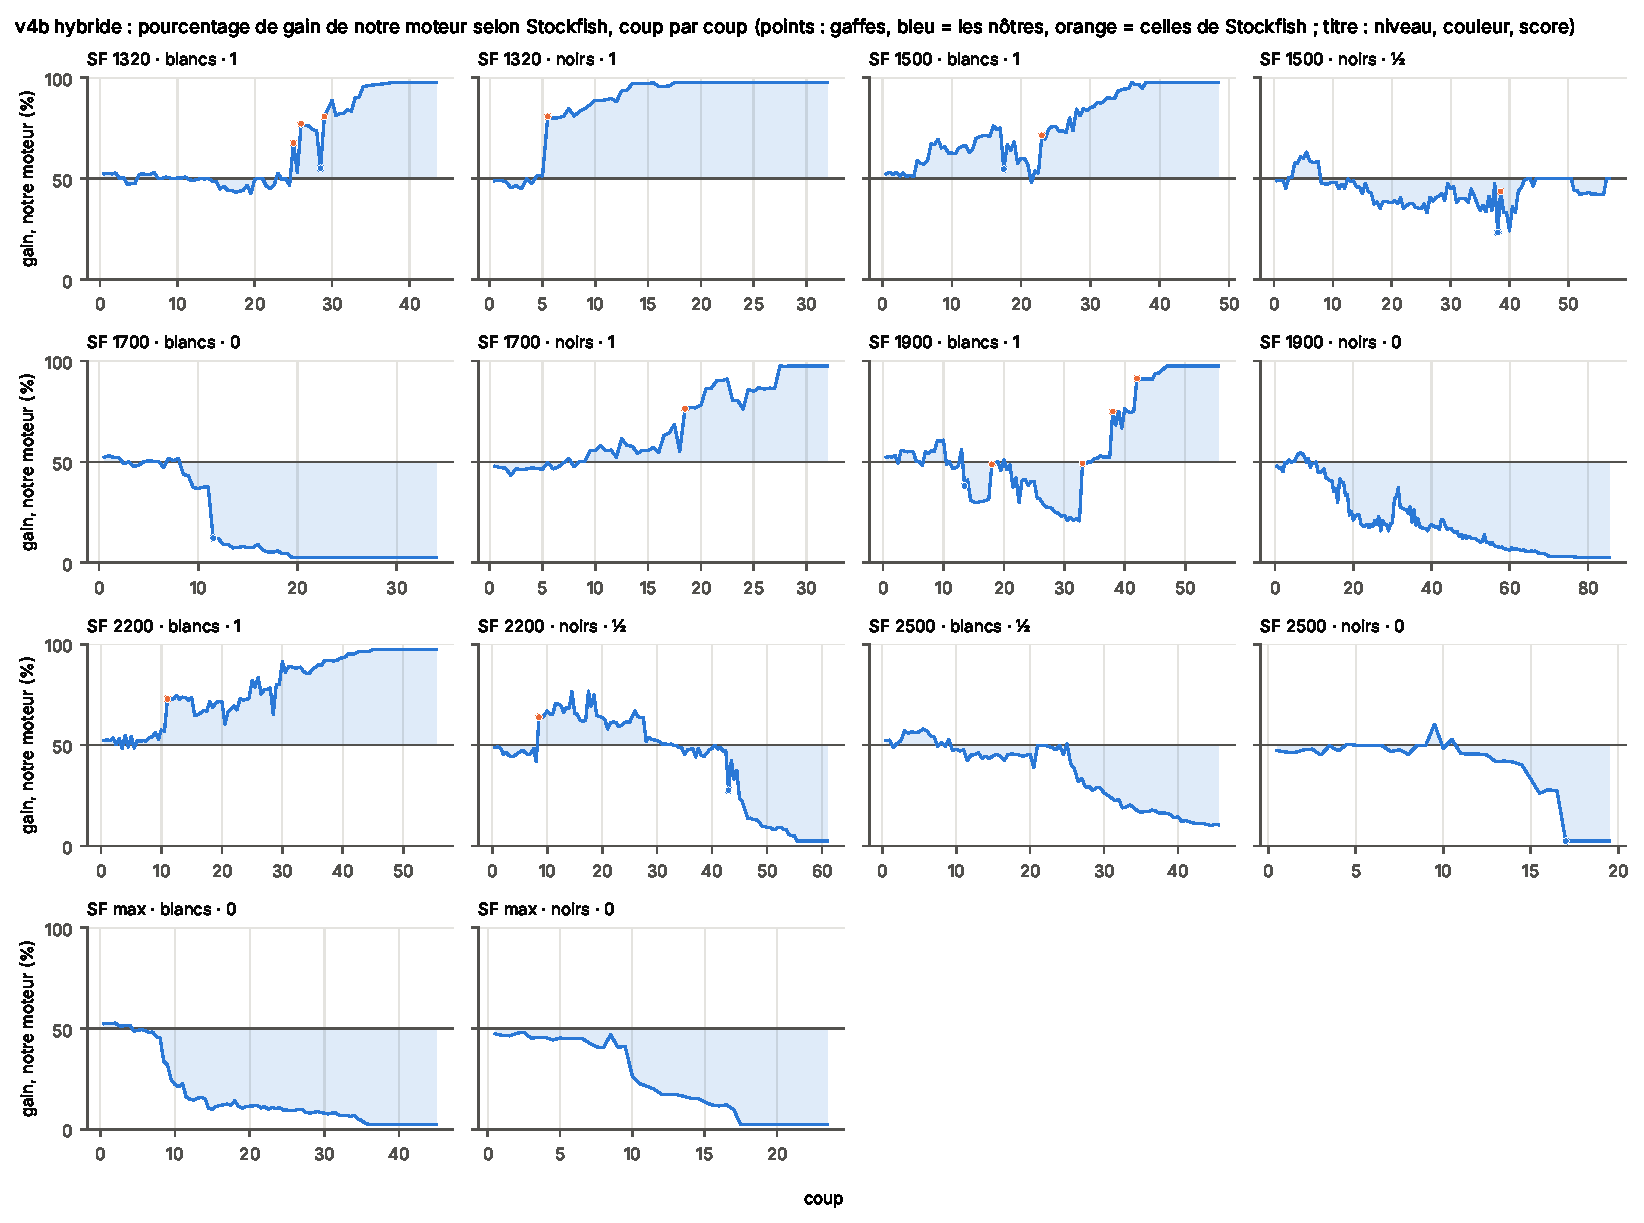
\includegraphics[width=\linewidth]{analyse/figs/courbes_v4b-hybride-ucielo-corrige.pdf}
\caption{Notre pourcentage de gain selon Stockfish, coup par coup, dans les 14 parties de l'alpha-bêta
hybride corrigé de l'incrément 1.}
\end{figure}

\paragraph{Lecture.} L'alpha-bêta corrigé est la série la plus précise : 93{,}5~\% de précision,
27~cp de perte moyenne et 0{,}5 gaffe par partie, contre 37{,}6~cp et 1{,}29 gaffe pour la pleine
largeur. C'est cohérent avec son 7{,}5/14. Nos coups se dégradent nettement aux coups 11 à 20 :
56~cp de perte et 5~\% de gaffes. Sur 36 défaites, le coup décisif tombe au coup 10{,}5 en
médiane, et il est de nous 35 fois sur 36. Les parties se perdent donc à la sortie de l'ouverture.

\section{Tri des coups et vagues adaptatives}
L'alpha-bêta par lots de l'incrément 1 triait les fils par évaluation statique. Trois tris sont
désormais disponibles :
\begin{itemize}
\item \code{statique}, celui de l'incrément 1 ;
\item \code{mvv}, qui joue d'abord les prises et les promotions, par victime décroissante puis par
attaquant croissant ;
\item \code{historique}, qui ajoute des coups « killer » par demi-coup et une table d'historique
mise à jour par \code{index\_add}.
\end{itemize}
Les vagues \code{adaptatif} choisissent, lot par lot, la découpe des fils selon la taille estimée
du sous-arbre (fils $\times$ branchement$^{\,rem-1}$). En dessous de $3\cdot10^4$, tout part d'un
coup ; jusqu'à $3\cdot10^7$, l'aîné puis le reste ; jusqu'à $3\cdot10^9$, la découpe hybride ;
au-delà, la découpe 1-2-4. Ces seuils ont été calibrés sur GPU ; leur optimum est plat et dépend de
la position.

\begin{table}[H]
\centering\small\begin{tabular}{lrrrrr}
\toprule
position & YBW stat. & hybride stat. & YBW MVV & adaptatif MVV & adaptatif hist.\\
\midrule
départ & 0{,}29~s & 0{,}78~s & 0{,}34~s & 0{,}30~s & 0{,}39~s\\
kiwipete & 1{,}30~s & 1{,}02~s & 1{,}03~s & 0{,}62~s & 0{,}74~s\\
italienne & 1{,}34~s & 1{,}86~s & 1{,}33~s & 0{,}66~s & 0{,}89~s\\
gambit-dame & 21{,}19~s & 2{,}23~s & 3{,}75~s & 1{,}12~s & 0{,}98~s\\
finale-tours & 0{,}60~s & 0{,}85~s & 0{,}55~s & 0{,}30~s & 0{,}38~s\\
\bottomrule
\end{tabular}

\caption{Temps mur à profondeur 6, quiescence 4, sur le pod de l'agent B. La valeur minimax est
identique dans chaque ligne.}
\end{table}

\paragraph{Ce qui compte.} Le tri MVV/LVA est le vrai gain : sur le Gambit-Dame, YBW passe de 21~s à
3{,}8~s. Les vagues adaptatives y ajoutent un facteur 1{,}5 à 2 sur quatre positions sur cinq. Les
coups « killer » et l'historique sont neutres, sauf sur le Gambit-Dame ; ils restent en option. Le
taux de coupe par l'aîné, désormais journalisé, passe de 0{,}38 à 0{,}76 sur le Gambit-Dame, et le
facteur de branchement effectif $N_6/N_5$ de 79 à 10.

\section{Pendule, répétition et journal}
\begin{itemize}
\item \textbf{Résultat partiel sûr.} Les coups racine sont cherchés par groupes 1, 1, 2, 4, 8\ldots
Interrompue, l'itération rend l'argmax des groupes terminés. C'est sûr dès que le premier coup a
fini : le coup rendu est soit lui, au score exact, soit un coup dont le score exact le dépasse. Un
test le prouve contre le minimax pleine largeur, avec et sans élagage.
\item \textbf{Plafond de temps à 1{,}5 fois le budget.} Sur CPU, la consommation maximale tombe de
4{,}1 à 1{,}6 fois le budget, sans perte de profondeur. Aucun prédicteur du coût de l'itération
suivante n'est fiable : l'erreur moyenne vaut un facteur 3. C'est le plafond, joint au résultat
partiel, qui borne le temps.
\item \textbf{Répétition.} Un coup racine qui ramène à une position déjà vue vaut 0. On l'évite
donc quand on mène et on le cherche quand on est perdu. Les répétitions plus profondes dans
l'arbre restent ignorées (\code{shortcut:}).
\item \textbf{Journal par coup} (\code{moves\_info}) : pour chaque coup, le score, la profondeur, les
nœuds, le temps et les pendules, de notre moteur comme de Stockfish.
\end{itemize}

\section{Validation sur GPU}
\subsection{Filtre de qualité}
On tire 100 positions des parties de l'incrément 1, avec une graine fixe. Chaque moteur dispose de
1~s par coup, et Stockfish juge le coup choisi en profondeur 16.
\begin{table}[H]
\centering\small\begin{tabular}{lrrrrr}
\toprule
moteur & perte moy. (cp) & médiane & $\ge 100$~cp & profondeur & temps (s)\\
\midrule
pleine largeur & 35{,}6 & 5 & 12~\% & 4{,}94 & 1{,}25\\
hybride, tri statique (incr. 1) & 35{,}9 & 5 & 12~\% & 5{,}02 & 0{,}88\\
adaptatif, tri MVV/LVA (incr. 2) & 29{,}6 & 4 & 8~\% & 5{,}91 & 0{,}99\\
\bottomrule
\end{tabular}

\caption{Perte du coup choisi par chaque moteur sur les mêmes 100 positions.}
\end{table}
Le nouveau moteur cherche presque un demi-coup plus profond et perd 6~cp de moins par coup. Il
choisit un coup perdant au moins 100~cp dans 8 positions sur 100, contre 12. Sur 100 positions,
cet écart reste indicatif.

\subsection{Duel de 200 parties}
Le nouveau moteur (vagues adaptatives, tri MVV/LVA) affronte l'ancien (vagues hybrides, tri
statique, c'est-à-dire l'alpha-bêta de l'incrément 1) en 10~s~+~0{,}1~s. Les 100 ouvertures sont
tirées au hasard sur 6 demi-coups et gardées si Stockfish les juge à moins de 60~cp ; chacune est
jouée deux fois, couleurs inversées. Les deux camps profitent de la pendule et du refus de la
répétition de l'agent C. Le duel mesure donc l'apport de la recherche (agent B), pas celui de la
pendule.

\begin{table}[H]
\centering\small\begin{tabular}{lr}
\toprule
mesure & nouveau / ancien\\
\midrule
parties & 200\\
score du nouveau moteur & 135/200 (67{,}5~\%)\\
victoires / nulles / défaites & 96 / 78 / 26\\
écart d'Elo (IC 95~\%) & $+127$ [$+90$ ; $+167$]\\
avec les blancs / les noirs & 66{,}5 / 68{,}5\\
profondeur moyenne (demi-coups) & 4{,}02 / 3{,}50\\
temps moyen par coup (s) & 0{,}23 / 0{,}19\\
nœuds par coup & 2443898 / 41203\\
coups au résultat partiel, par partie & 10{,}47 / 1{,}44\\
pendule minimale (s) & 3{,}20 / 5{,}06\\
\bottomrule
\end{tabular}

\caption{Duel de 200 parties : score, Elo et comportement moyen par partie.}
\end{table}

\begin{figure}[H]
\centering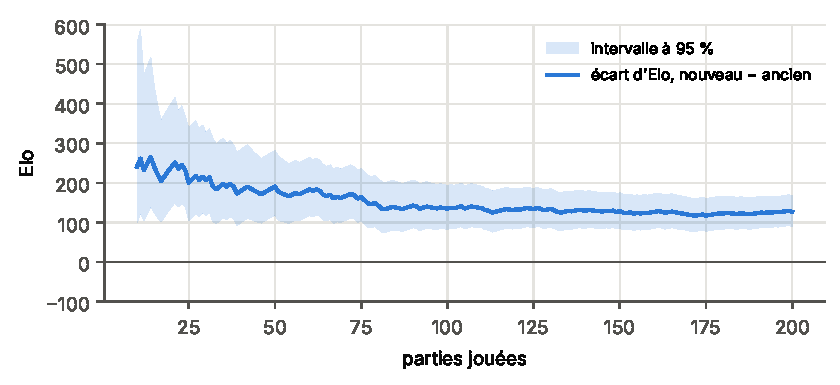
\includegraphics[width=0.85\linewidth]{figs/duel_elo.pdf}
\caption{Écart d'Elo cumulé au fil du duel et son intervalle à 95~\%.}
\end{figure}

\begin{table}[H]
\centering\footnotesize\begin{tabular}{lrrrrr}
\toprule
moteur & précision (\%) & perte (cp) & erreurs/partie & gaffes/partie & coups décisifs\\
\midrule
nouveau (adaptatif, MVV/LVA) & 89{,}2 & 51{,}3 & 2{,}58 & 3{,}05 & 32\\
ancien (hybride, statique) & 87{,}9 & 58{,}9 & 2{,}96 & 3{,}31 & 90\\
\bottomrule
\end{tabular}

\caption{Les 200 parties du duel analysées par Stockfish en profondeur 14. « Coups décisifs » : le
camp qui a joué le coup après lequel la partie était jouée (parties décisives seulement).}
\end{table}

\paragraph{Lecture.} Le nouveau moteur gagne nettement : $+127$ Elo, avec un intervalle de $+90$ à
$+167$ qui exclut zéro de loin. Le résultat est équilibré entre les couleurs (66{,}5 et 68{,}5 points
sur 100). Il calcule 60 fois plus de nœuds par coup pour un temps proche, ce qui montre que le tri
MVV/LVA remplit mieux les lots GPU. Il ne perd jamais au temps, malgré une dizaine d'itérations
interrompues par partie, toutes rattrapées par le résultat partiel. Ses coups sont plus précis, et
l'ancien moteur commet 90 des 122 coups décisifs. En 10~s~+~0{,}1~s, les deux moteurs ne cherchent
qu'à 3{,}5 à 4 demi-coups, d'où une précision absolue modeste, autour de 88 à 89~\%.

\section{Limites}
\begin{itemize}
\item Le duel est une partie contre soi-même : un écart d'Elo entre deux versions d'un même moteur
surestime en général l'écart contre un adversaire tiers. L'Elo contre Stockfish reste à mesurer.
\item Le duel ne mesure pas l'apport de l'agent C, présent dans les deux camps.
\item Les coups des 200 parties du duel et le détail coup par coup de leur analyse sont restés sur le
pod et ont été perdus à sa suppression. Seules les synthèses par partie sont archivées, dans
\code{donnees/}.
\item Les formules de Lichess ont été reprises de mémoire par l'agent A, et la colonne Stockfish de
l'analyse mélange des niveaux bridés qui commettent des erreurs exprès.
\item Les seuils des vagues adaptatives ont été calibrés sur trois positions seulement.
\end{itemize}

\section{Plan du prochain incrément}
\begin{enumerate}
\item \textbf{Mesurer contre Stockfish} le moteur de l'incrément 2, en préréglage \code{uci-elo},
avec 50 parties par niveau autour de 1500 à 2200. C'est le seul Elo comparable à l'extérieur.
\item \textbf{Renforcer la sortie de l'ouverture}, là où l'analyse localise les pertes (coups 11 à
20) : sécurité du roi, mobilité et développement dans l'évaluation, ou un petit livre
d'ouvertures. Validation : la perte par tranche de coups, puis un duel.
\item \textbf{Table de transposition sur GPU} : réutiliser le meilleur coup d'une itération à
l'autre aux niveaux internes, et détecter les répétitions dans l'arbre.
\item \textbf{Élagage non exact} (LMR, coup nul), validé par duel puisque l'égalité avec le
minimax ne tiendra plus.
\item \textbf{Volet rétrograde} : imposer une condition finale, comme le mat étouffé, par
préimages sur GPU.
\end{enumerate}

\section{Reproductibilité et coûts}
{\footnotesize
\begin{verbatim}
python -m unittest src.matrix_chess.test_gpu_engine src.matrix_chess.test_search_control \
                   src.matrix_chess.test_analyse src.matrix_chess.test_duel
python -m src.matrix_chess.analyse parties <games.txt> --sortie DOSSIER
python -m src.matrix_chess.analyse filtre <games.txt> -n 100 --budget 1 \
       [--prune --waves adaptatif --tri mvv]
python -m src.matrix_chess.duel --a "prune=1,waves=hybride,tri=statique" \
       --b "prune=1,waves=adaptatif,tri=mvv" -n 100 --clock 10 --inc 0.1
python docs/etudes/2026-11-24_increment2/gen_figures.py
python docs/etudes/2026-11-24_increment2/analyse/gen_figures.py
\end{verbatim}}

L'incrément a utilisé un seul pod RTX PRO 6000 à 2{,}69~\$/h, d'abord pour la mise au point de
l'agent B, puis pour la validation. Il a coûté 5{,}90~\$ (solde passé de 52{,}93 à 47{,}03~\$), et
le pod a été supprimé.

\end{document}
